% ============================================
%  Article Class (This is a LaTeX2e document)  
% ============================================
\documentclass[12pt]{scrartcl}

\usepackage[english]{babel}
\usepackage[utf8]{inputenc}

\usepackage{enumitem}
\usepackage[round]{natbib}
\usepackage{color}

\newcommand\reft[3][]{#2~\ref{#3}#1}
\newcommand\refp[3][]{(#2~\ref{#3}#1)}
\newcommand\refsect[1]{\reft{Section}{#1}}
\newcommand\refsecp[1]{\refp{Sec.}{#1}}
\newcommand\reftabt[1]{\reft{Table}{#1}}
\newcommand\reftabp[1]{\refp{Tab.}{#1}}

% ======
%  Math
% ======
\usepackage{amsmath}
\usepackage{amsthm}
\usepackage{mathtools} % \mathclap
\newtheorem{thm}{Theorem}[section]
\newtheorem{cor}[thm]{Corollary}
\newtheorem{lem}[thm]{Lemma}
\newtheorem{prop}[thm]{Proposition}
\newtheorem{property}[thm]{Property}
\theoremstyle{definition}
\newtheorem{defn}[thm]{Definition}
\newtheorem{assum}[thm]{Assumption}
\theoremstyle{remark}
\newtheorem{rem}[thm]{Remarque}
\numberwithin{equation}{section}

\usepackage{amssymb}
\newcommand{\prob}[1]{\mathbb{P}\left(#1\right)}
\newcommand{\Ker}[1]{\mathrm{Ker}\left(#1\right)}
\newcommand{\Image}[1]{\mathrm{Im}\left(#1\right)}
\newcommand{\diag}[1]{\mathrm{diag}\left(#1\right)}
\newcommand{\Vect}[1]{\mathrm{Vect}\left\{#1\right\}}

% ============================
%  Figures and relative paths
% ============================
\usepackage{graphicx}
\graphicspath{{figures/}}
\usepackage{import}
\makeatletter
  \def\relativepath{\import@path}
\makeatother
\newcommand\reffigt[2][]{\reft[#1]{Figure}{#2}}
\newcommand\reffigp[2][]{\refp[#1]{Fig.}{#2}}

% ==========
%  Document
% ==========
\begin{document}

\title{RBA}%
\author{S. Fischer - Biosys - MAIAGE}%
\date{\today}%

\maketitle

\newpage

\tableofcontents

\newpage

\section{Principles underlying algorithm}

\reffigt{fig:rba} shows how the fluxes of molecules are described by RBA and where the constraint are placed.

\begin{figure}[ht]
  \centering
  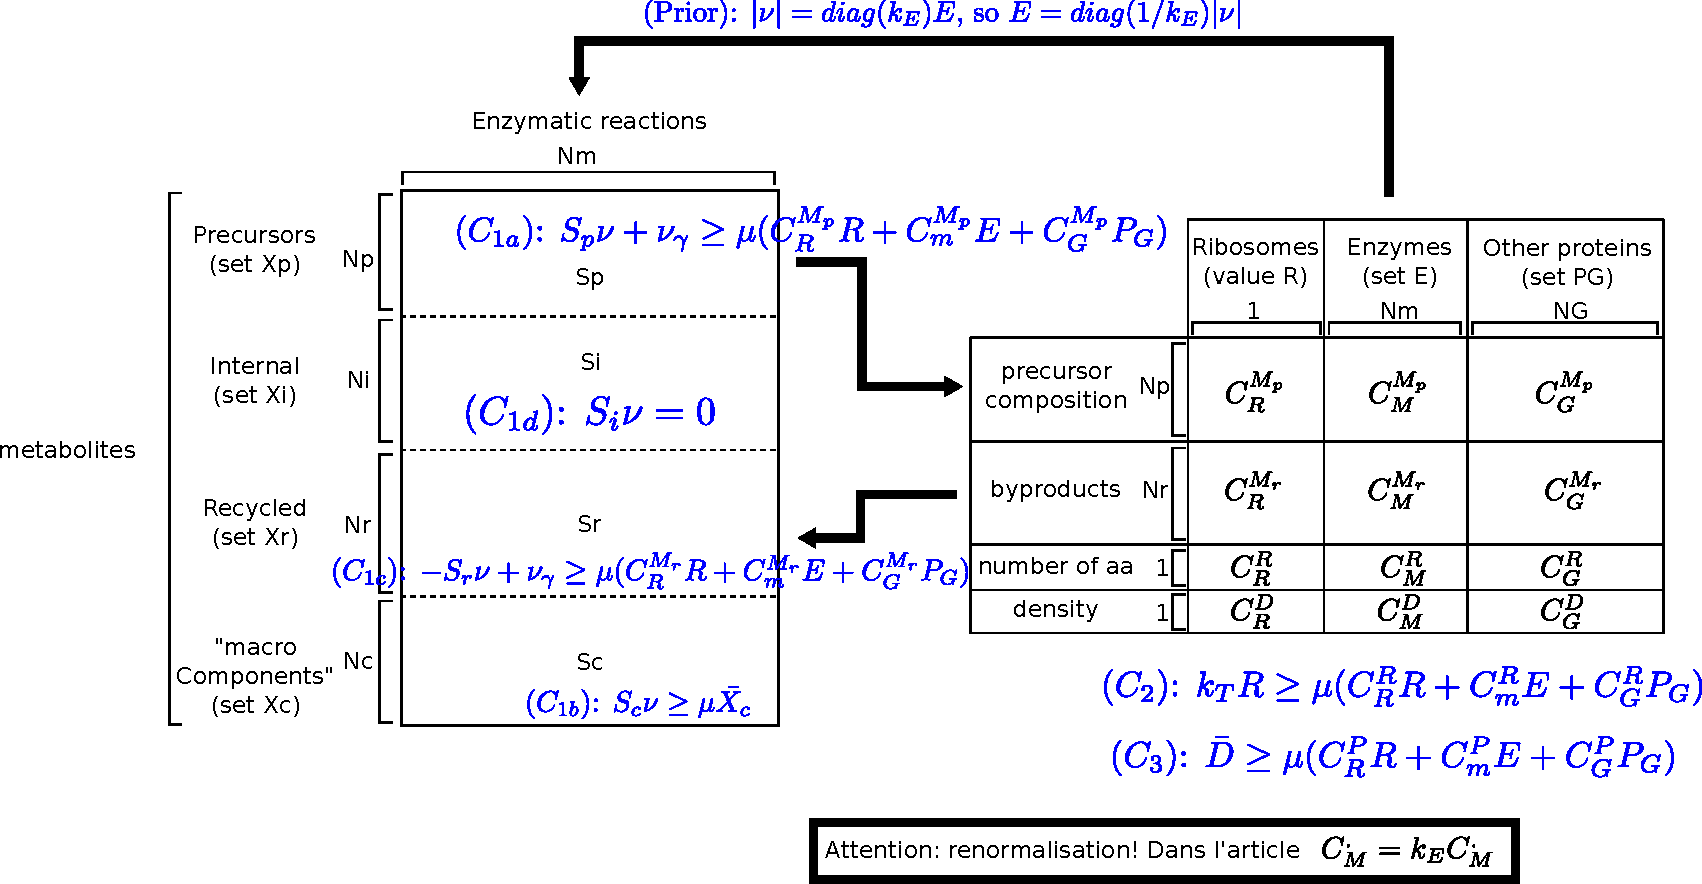
\includegraphics[width=\linewidth]{RBA}
  \caption{Description of cell by RBA.}
  \label{fig:rba}
\end{figure}

\section{Analysis of existing algorithm (RBAV01)}

\subsection{Structure of RBAV01}
The original program is built around a multitude of functions and structures displayed on~\reffigt{fig:algo_rba}. \reffigt{fig:matrices_rba} shows how matrices are built in the original algorithm.

\begin{figure}[ht]
  \centering
  \includegraphics[width=\linewidth]{algo_RBA}
  \caption{Algorithm used in RBAV01.}
  \label{fig:algo_rba}
\end{figure}

\begin{figure}[ht]
  \centering
  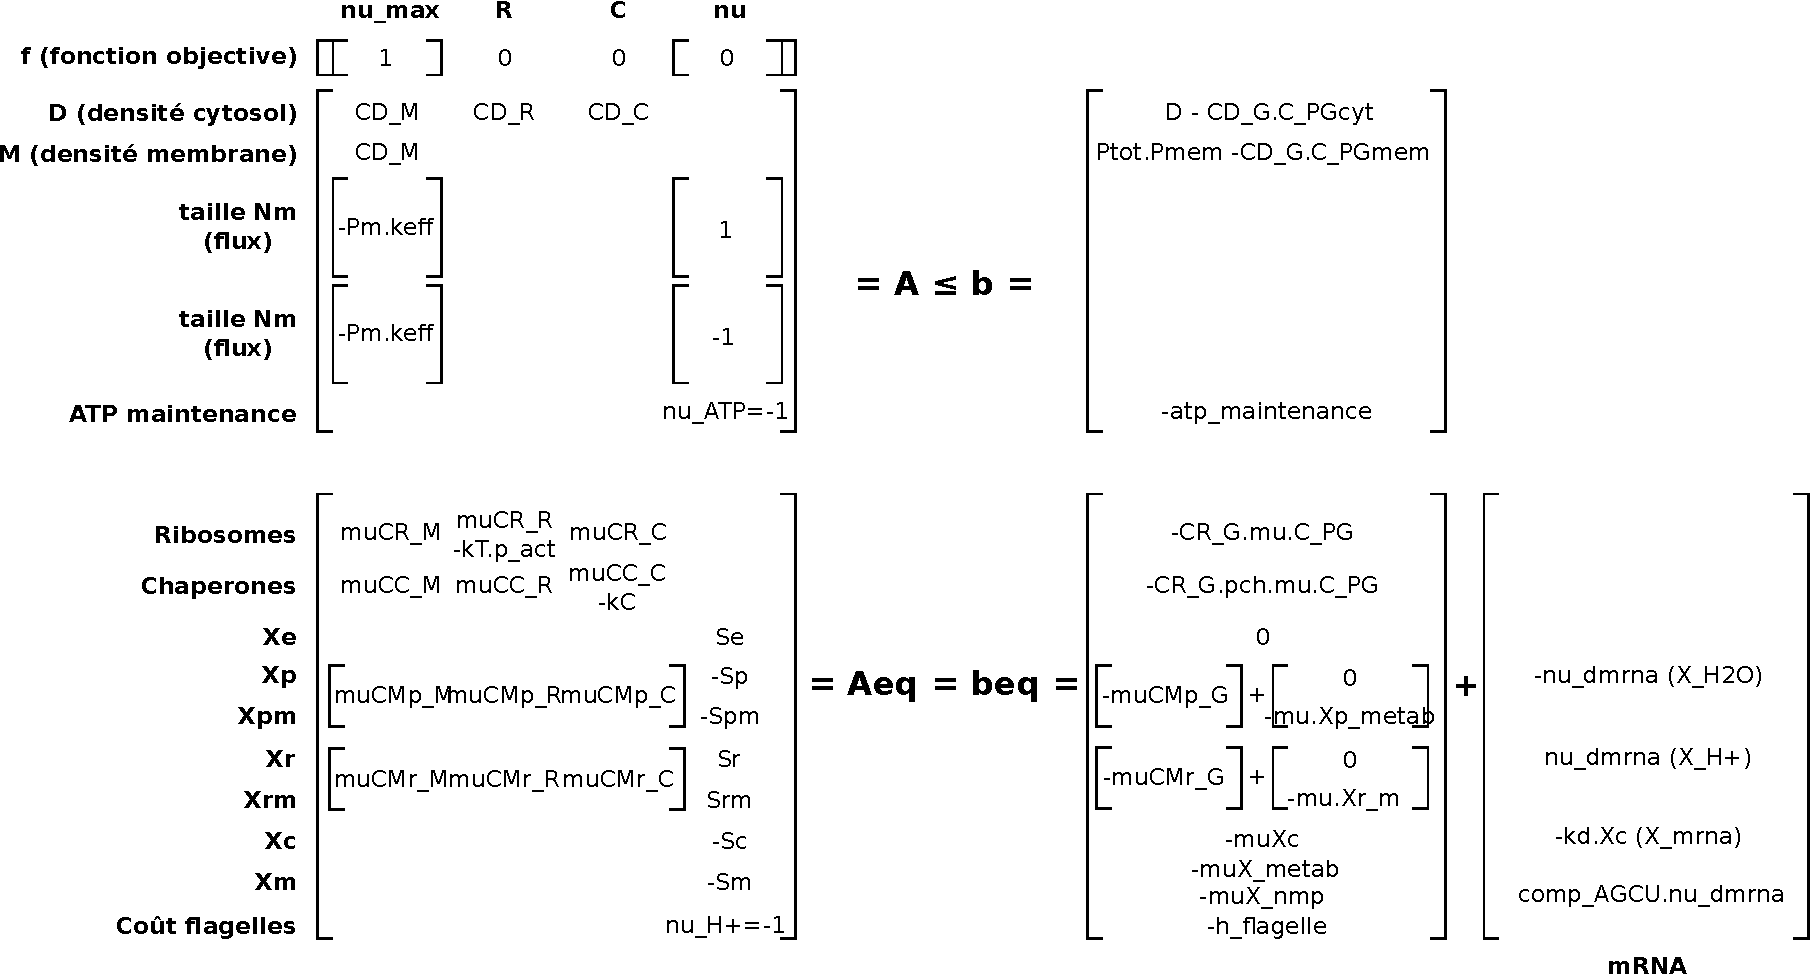
\includegraphics[width=\linewidth]{matrices_RBA}
  \caption{Matrices used in RBAV01.}
  \label{fig:matrices_rba}
\end{figure}

\clearpage

\subsection{Orientations for improving RBA algorithm}

It would be more elegant and flexible to not name any metabolite or flux sets. These sets should be defined by data, not the program. The existence of $X_{e/c/r/rm/p/pm/m}$ is unnecessary. Note that there are even more subsets than defined in theory, we probably need to avoid proliferation of such subsets.

We need to find clear abstraction that can represent RBA entities as generically as possible. All macromolecules should be representable with a composition matrix that would help build the final matrices rapidly. We also need to express the second member as data, in terms of processes.

Final objectives are
\begin{itemize}
\item Completely separate data from code: Create data files that are meaningful to users.
\item Make code more compact and easier to read (and potentially quicker): by using a full matrix formalism (avoiding loops). This can only be achieved by finding the right abstraction to represent RBA elements.
\end{itemize}

\clearpage
\section{Rewriting RBAs in full matrix form}

\paragraph{Composition vector for macromolecules} In the following, each macromolocule is described by its \textbf{composition vector}. It is a column vector containing the metabolites necessary to build it, with a \textbf{minus} sign for metabolites consumed and a \textbf{plus} sign for byproducts generated.

\paragraph{Metabolism constraint} The metabolism constraint $(C_1)$ can be rewritten

\[
\overbrace
{
\underbracket{S\nu}_{\parbox{2cm}{\scriptsize metabolic flux generated by metabolism}} 
+
\underbracket{\mu [C_E,C_R,C_C] [E;R;C]}_{\parbox{3cm}{\scriptsize precursors used/byproducts generated by producing new molecules}}
}^{\text{\normalsize `Variable' terms}}
=
\overbrace
{
\underbracket{-\mu [C_{G},C_{X_c}] [P_G;X_c]}_{\parbox{3cm}{\scriptsize precursors used/byproducts generated by producing new molecules}}
}^{\text{\normalsize Constant terms}} \\
\]
\[
-\diag{k_E} E \leq \nu \leq \diag{k_E} E
\]

where $C_{i}$ are composition matrices as defined above.

Written this way, it actually does not matter to which group a metabolite belongs. Its group is only dictated by the structures of the composition matrices. Based on this constraint only it does not make sense to create metabolic groups \emph{in the program}.

In full matrix form, the above equations become
\[
\left\{
\begin{array}{ccc}
  [S, \mu C_E, \mu C_R, \mu C_C][\nu;E;R;C]
  & = & - [\mu C_G,\mu C_{X_c}][P_G;X_c] \\
  \left[
    \begin{array}{cccc}
      I, & -\diag{k_E}, & 0, & 0 \\
      -I, & -\diag{k_E}, & 0, & 0
    \end{array}
    \right]
       [\nu; E;R;C] &\leq & 0
\end{array}
\right.
\]

The most important here is the composition matrix. In the data, the user gives the list of metabolites used for synthesis and the list of byproducts. The program then has to figure out how to reorder terms to build the matrix.

\paragraph{Ribosome/chaperone constraints} We can rewrite the ribosome constraint as follows:
\[
k_TR + \mu [C^R_E,C^R_R,C^R_C] [E;R;C] = -\mu C^R_GP_G
\]
In full form:
\[
[0,\mu C^R_E,k_T+\mu C^R_R,\mu C^R_C] [\nu;E;R;C] = [-\mu C^R_G,0][P_G;X_c]
\]

The number of aas needed to build a protein can be included in the description of molecule sets. The same applies for folding by chaperones. 

These additionnal constraints have the form
\[
a [\nu; E; R; C] = b_0 + b_1 [P_G;X_c]
\]
this means they can be appended to $C_1$ by \textbf{simple line concatenation}.

\paragraph{RNA degradation/replication} In this type of constraints, we simply add new fluxes of metabolites. These fluxes are simply added up on the right hand side of $(C_1)$
\[
\begin{array}{rcl}
...  & = & -\mu[C_G,C_{X_c}][P_G;X_c] - \mu^{d}C_{process}X_{process} \\
 & =  & -[\mu C_G, \mu C_{X_c},\mu^d C_{process}][P_G;X_c;X_{process}]
\end{array}
\]
where $d = 0$ when the target flux is an abolute flux and $d=1$ when it compensates dilution.

\paragraph{Density constraints} The density constraint writes
\[
[0,C^D_E,C^D_R,C^D_C] [\nu;E;R;C] \leq \overline{D} - [C^D_G,C^c_G][P_G;X_c]
\]
In general, these constraints can be expected to be of the form
\[
a [\nu; E; R; C] \leq b_0 + b_1 [P_G;X_c]
\]

\paragraph{Maintenance ATP constraint (metabolite specific constraints)} It is defined as
\[
\mathbf{1}_{\nu_{constraint}} [\nu; E; R; C] = b
\]
where $\mathbf{1}_{\nu_{constraint}}$ is an indicator matrix selecting the reaction associated with the production of maintenance ATP/flagella fuel. Generally this means a specific reaction has to be added in $S$, as well as specific metabolites like ATP maintenance or protons dedicated to fuelling flagella.

\paragraph{Summary}

\[
\begin{array}{ccll}
  [S, \mu C_E, \mu C_R, \mu C_C] & [\nu;E;R;C] = & 
  - \sum \mu^{d_i}C_i X_i & \textrm{(Base metabolism}\\
  & & & \textrm{and process production)} \\
  a & [\nu; E; R; C] = & b_0 + b_1 [\{X_i\}] & \textrm{(Process capacity)}\\
  \mathbf{1}_{\nu_{constraint}} & [\nu; E; R; C] = & b & \textrm{(Metabolite constraints)} \\
  \left[
    \begin{array}{cccc}
      I, & -\diag{k_E}, & 0, & 0 \\
      -I, & -\diag{k_E}, & 0, & 0
    \end{array}
    \right] & [\nu; E;R;C] \leq & 0 & \textrm{(Enzymatic fluxes)}\\
  a & [\nu; E; R; C] \leq & b_0 + b_1 [\{X_i\}] & \textrm{(Density constraints)} \\
\end{array}	
\]

A more graphic representation of the matrix is provide in \reffigt{fig:new_matrices_rba}.

\begin{figure}[ht]
  \centering
  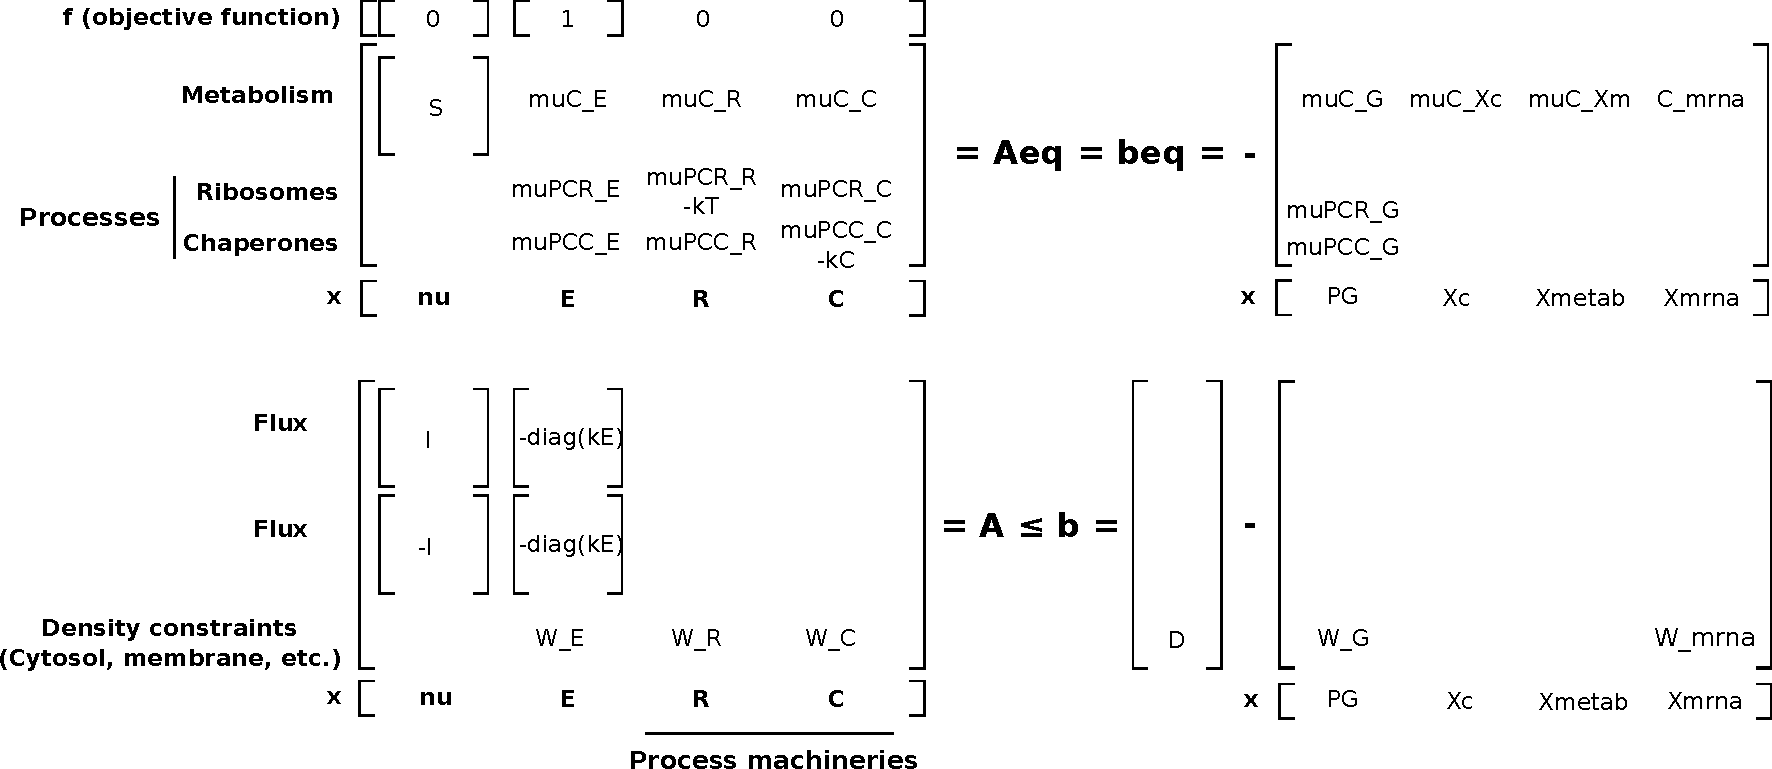
\includegraphics[width=\linewidth]{new_matrices_RBA}
  \caption{Structure of matrices. Note that the left hand side and the right hand side have a similar structure (except for the $\nu$ submatrix). Each column represents a set of molecules: on the right hand side, the production flux of the set has to be determined, on the left hand side it is already given \textit{a priori}.}
  \label{fig:new_matrices_rba}
\end{figure}

\clearpage
\section{New formalism}

The new formalism must allow simple interactions between user readable data and ifficient construction of the RBA problem. The data is going to be written is XML format, inspired by SBML standards.

\subsection{Final differences between RBAv01 and new formalism}

\begin{table}[!h]
  \centering
  \begin{tabular}{|l|c|c|c|c|}
    \hline
           & RBAv01 & RBAv01 & RBAnew \\
           & mat12  & mat15  & python \\
    \hline
    Input files & \multicolumn{2}{c|}{Custom files} & XML files \\
    & \multicolumn{2}{c|}{+ partially hard coded} & (nothing hard coded) \\
    \hline
    Code length & \multicolumn{2}{c|}{$\simeq 3500$} & $\simeq 2000$ \\
    (commented) & \multicolumn{2}{c|}{($\simeq 1000$)} & ($\simeq 500$) \\
    \hline
    Parsing & 15s & 8s & $<1$s \\
    \hline
    Solving (23 rounds) & 15s & 5s & $<2$s \\
    \hline
    1 matrix update & 580ms & 100ms & 3-10ms \\
    \hline
    1 CPLEX round & 50ms & 58ms & 30ms \\
    \hline
  \end{tabular}
  \caption{Comparison between original algorithm (RBAv01) and new formalism (RBAnew). Because performance for the old algorithm depended on matlab version, we included performance for matlab R2012a (mat12) and R2015b (mat15).}
  \label{tab:new_old_comparison}
\end{table}

\reftabt{tab:new_old_comparison} shows the main differences between RBAv01 and the new algorithm. The new algorithm uses generic XML files and is thus easier to modify for the end user. Using python, we could improve both parsing and solving time, which are significantly lower than the original algorithm.

\subsection{Input data}
Data files are described in Appendix~\ref{sec:rba_xml}.

\subsection{From data to matrices}

\paragraph{Algorithm overview}
\reffigt{fig:algo_rba_new} shows the blocks that are used to build the final matrices.
\begin{figure}[ht]
  \centering
  \includegraphics[width=\linewidth]{algo_RBA_new}
  \caption{Blocks that need to be assembled in the new algorithm.}
  \label{fig:algo_rba_new}
\end{figure}

\paragraph{Stoichiometry matrix} The procedure is standard, we will not illustrate it here. However, note that external metabolites are removed from the metabolite pool.

\paragraph{Density limits} These values are simply extracted from RBAParameters and assembled into a vector (one coefficient per compartment).

\paragraph{Species matrices} \reffigt{fig:species_matrices} shows how macromolecules are breaken down into matrices describing their composition, processing cost and weight. In the end, they are merged into a single matrix describing composition, processing cost and weight of all metabolites and macromolecules.
\begin{figure}[ht]
  \centering
  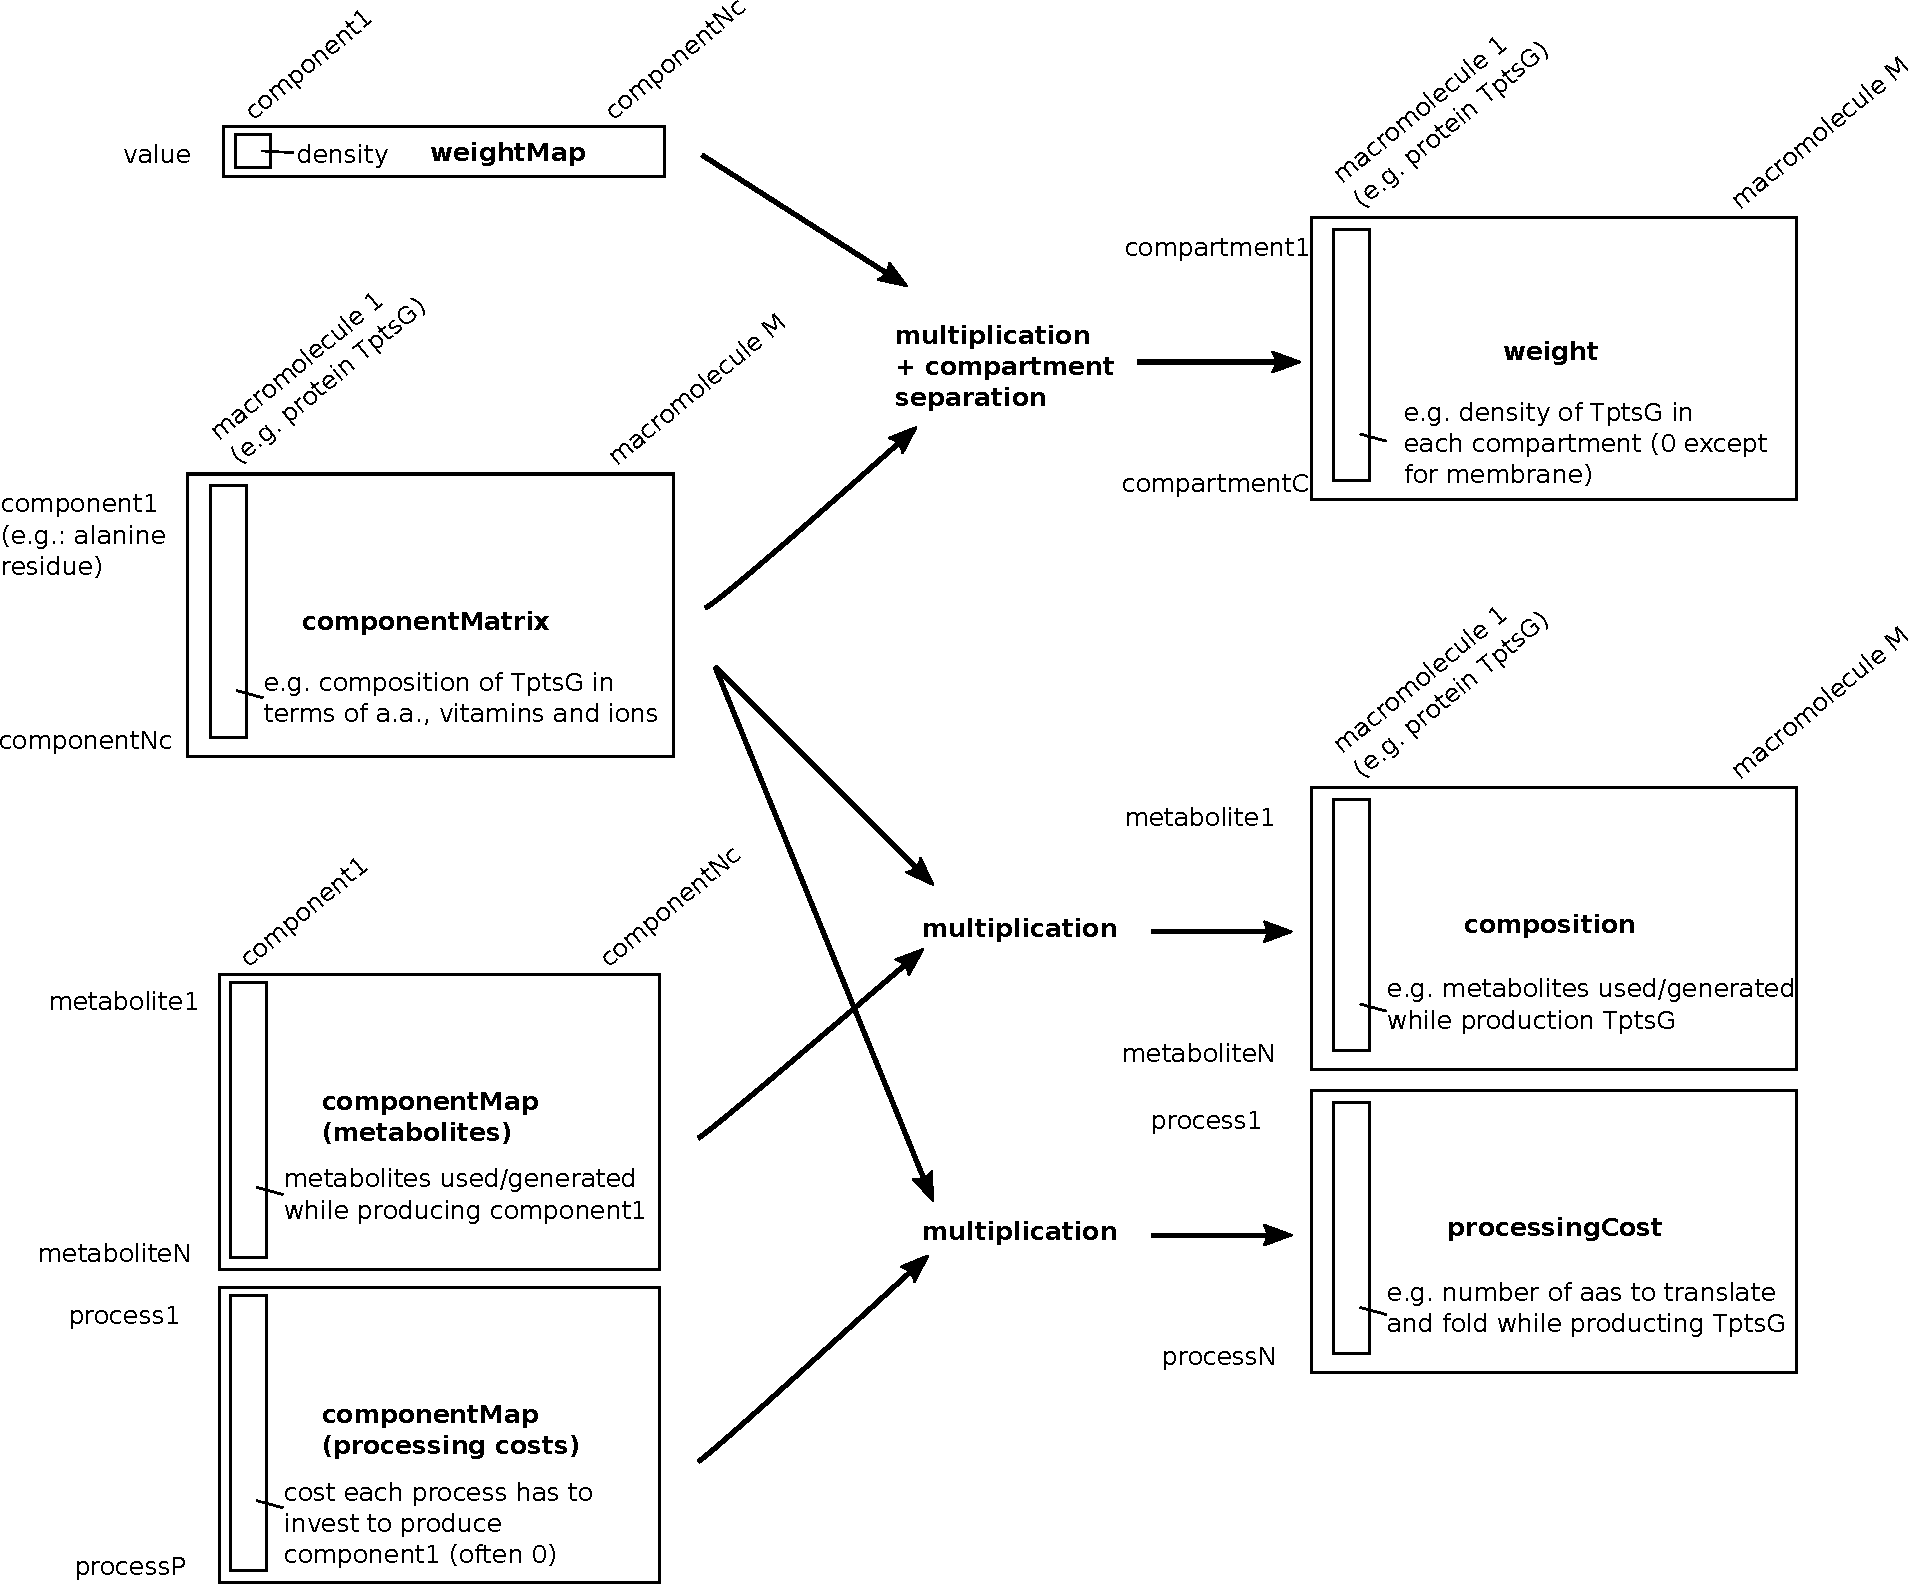
\includegraphics[width=\linewidth]{species_matrices}
  \caption{Matrices extracted from macromolecule information. An example is given with proteins but in the end, they contain all macromolecules and all internal metabolites.}
  \label{fig:species_matrices}
\end{figure}

\paragraph{Machinery matrices} \reffigt{fig:machinery_matrices} shows how the matrices stored in \texttt{rba.processes} are built.
\begin{figure}[ht]
  \centering
  \includegraphics[width=\linewidth]{machinery_matrices}
  \caption{Every machinery can be described by a reaction matrix. Reactants are species (metabolites or macromolecules) needed to build the machinery and products are byproducts of the assembly process. Through matrix multiplication with the species matrices, we can deduce its composition, weight and processing cost.}
  \label{fig:machinery_matrices}
\end{figure}

\paragraph{Target matrices} Targets are either metabolites or macromolecules. Their composition, processing cost and weight can be extracted as columns from the species matrices.


\clearpage

\appendix

\section{RBA XML}
\label{sec:rba_xml}

\paragraph{Metabolism file}
\begin{figure}[ht]
  \centering
  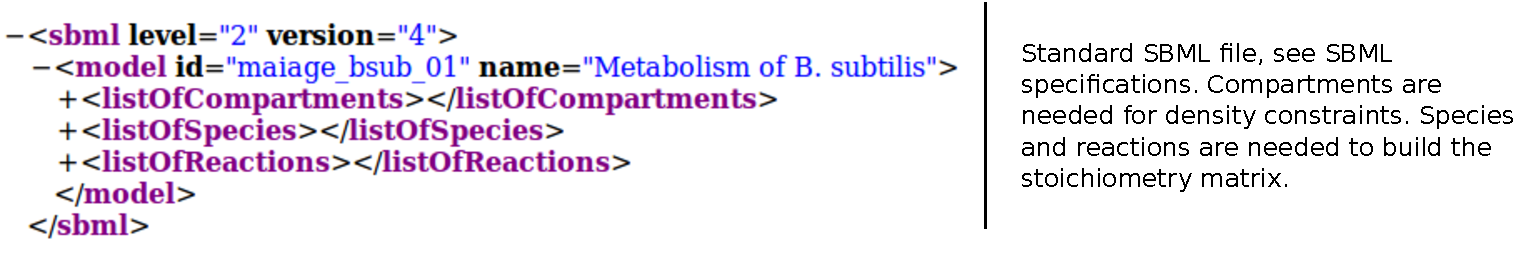
\includegraphics[width=\linewidth]{metabolism}
  \caption{Metabolism file is a standard SBML file.}
  \label{fig:metabolism}
\end{figure}
The metabolism file is a standard SBML file~\reffigp{fig:metabolism}. It contains information about cell compartments, metabolite species and metabolism reactions. Concentration of external metabolites are defined in the species section.

\paragraph{Parameter file}
\begin{figure}[ht]
  \centering
  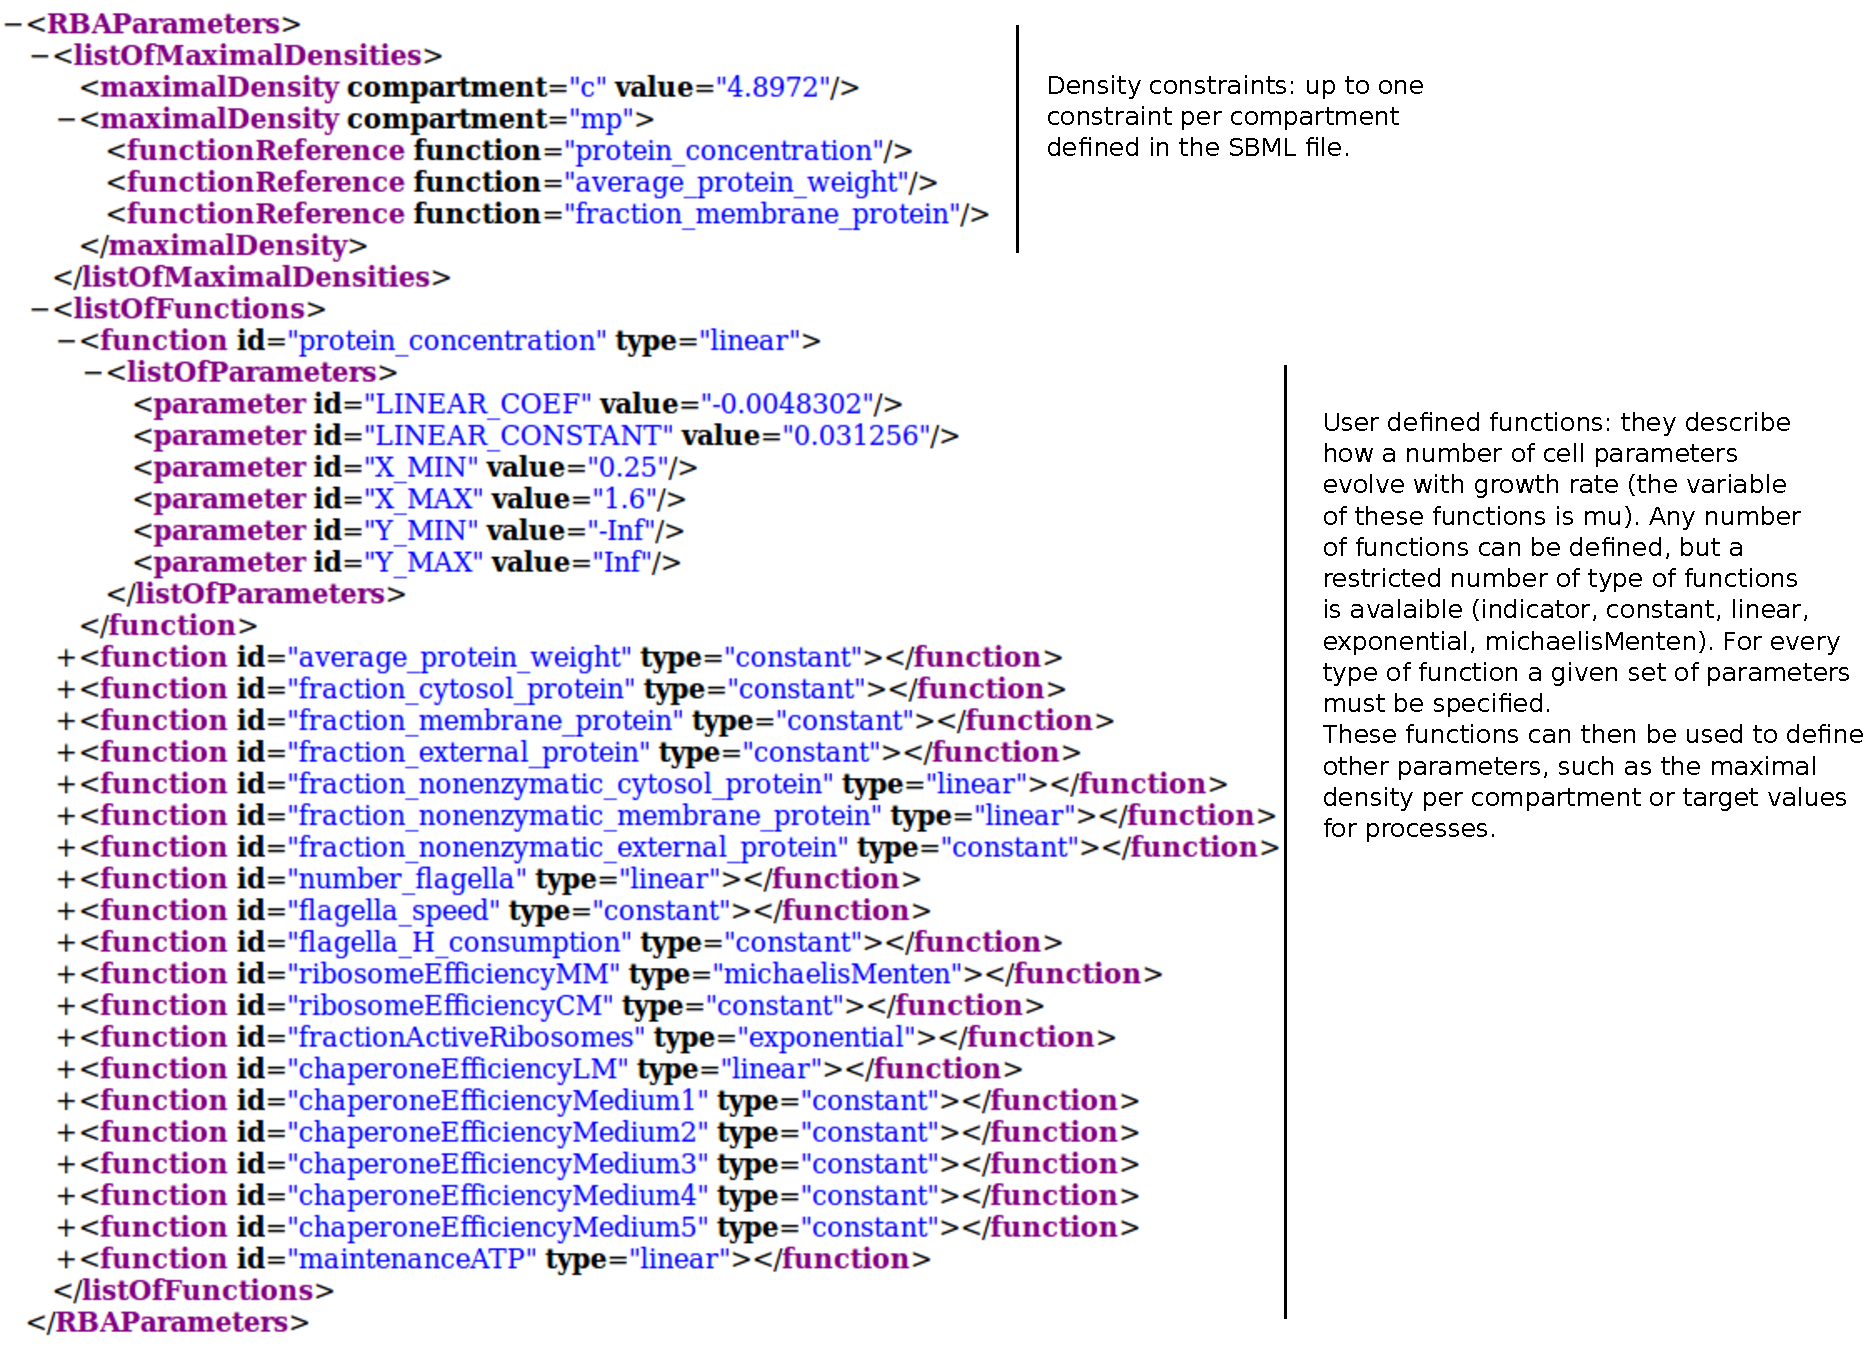
\includegraphics[width=\linewidth]{parameters}
  \caption{Structure of the parameter file used by RBA.}
  \label{fig:parameters}
\end{figure}
The parameter file is an XML file composed of two subsections~\reffigp{fig:parameters}. \texttt{listOfMaximalDensities} contains density constraints. \texttt{listOfFunctions} contains user-defined functions that can be used to set $\mu$-dependent maximal densities or $\mu$-dependent process targets (see below).

\paragraph{Macromolecule files}
\begin{figure}[ht]
  \centering
  \includegraphics[width=\linewidth]{proteins}
  \includegraphics[width=\linewidth]{rnadna}
  \caption{Structure of protein, RNA and DNA file.}
  \label{fig:proteins}
\end{figure}
Currently, RBA defines three sets of macromolecules: proteins, RNAs and DNA. One XML file is created for each set~\reffigp{fig:proteins}. All macromolecules have a \texttt{listOfComponents} describing the building blocks used to produce them (\textit{e.g.} amino acids, vitamins and ions for proteins). Then a \texttt{listOfSpecies} contains all molecules of the set, including their description in terms of components. Additionally, proteins have a \texttt{listOfEfficiencyFunctions} that lists efficiency models for enzymes. Enzymes contain an \texttt{enzymaticActivity} structure that defines the reaction they catalyze and the parameters for the efficiency models. Finally, transporters have a \texttt{transporterEfficiency} that modulates the enzymatic activity depending on substrate and cofactor availability.

\paragraph{Process file}
\begin{figure}[ht]
  \centering
  \includegraphics[width=\linewidth]{processes}
  \caption{Structure of process file.}
  \label{fig:processes}
\end{figure}
The process file is an XML file containing a \texttt{listOfProcesses} and a \texttt{listOfComponentMaps}. Each \texttt{process} can contain up to 3 subsections. The \texttt{capacityConstraint} defines a machinery used by the process that has a limited capacity. The \texttt{operatingCosts} defines which macromolecules the process produces/degrades/modifies and the cost associated with these operations. The \texttt{targets} are set fluxes that a process must maintain in order for the cell to work properly. Target fluxes can apply to metabolites (\texttt{targetValue}) and reactions (\texttt{targetReaction}). Target fluxes scale with $\mu$ if they contribute to \texttt{dilution\_compensation} or if they are defined using a $\mu$-dependent user-function. Finally \texttt{componentMaps} are used to compute the costs in the \texttt{operatingCosts} section.


\section{Small bug in RBAv01}

There was a slight bug in RBAv01. A typo in indexing while updating transporters
had the following consequences:
\begin{itemize}
\item Two Fe transporter would not be initialized properly. They worked at default capacity. In the presence of Fe, this has only a low impact as they would be active anyway. In the absence of Fe, they would keep working.
\item Instead, the catalytic efficiency of enzyme EPtsI was modified. In the presence of Fe, it would divide its catalytic activity by 2, leading to slightly lower growth rate than expected (something like 0.015). In the absence of Fe, the forward reaction catalyzed by EPtsI would be blocked.
\end{itemize}

Briefly, this bug has a small impact in the presence of Fe and a dramatic impact in the absence of Fe. To our knowledge, there is no dataset where Fe was removed from the medium, explaining why this bug has not been discovered earlier.


%\bibliographystyle{myplainnat}
%\bibliography{biblio}

\end{document}
% ----------------------------------------------------------------
